\chapter{The Histogram of Gradient Orientations of Signal Plots}
\label{chapter:three}

This Chapter introduces the EEG feature extraction procedure based on the Histogram of Gradient Orientations.  This method is grounded on an extension and modification of the SIFT~\cite{Lowe2004} Descriptor which is used in Computer Vision to extract and map local regions of an image.  At the same time, this Chapter brings to completion the previous one, describing how to mine the information from a plot and build a feature out of it.

\section{Introduction}

%sinuplot, spectrogram, scalogram

The work of Edelman, Intrator and Poggio~\cite{Edelman1997} on how the visual cortex sense features was the inspiration to the development of an algorithm to identify and decode salient local information from image regions.  The Scale Invariant Feature Transform (SIFT) method is composed of two parts, the SIFT Detector and the SIFT Descriptor.  The first is the procedure to identify relevant areas of an image.  The second is the procedure to describe and characterize a region of an image (patch) using the Histogram of Gradient Orientations~\footnote{It should not to be confused with HOG~\cite{Dalal2005}, the Histogram Of Gradients which is another method from Computer Vision based on similar ideas.  Actually, the descriptor part of the SIFT Method has no specific name, but it is based on building a histogram of gradient orientations.}.  The SIFT algorithm is biomimetically inspired in how the visual cortex detects shapes by analyzing orientations~\cite{Edelman1997}.  The patch description is also based on the Theory of Receptive Fields and other related ideas~\cite{Lindeberg2013}.

\pagebreak

\section{Feature Extraction: Histogram of Gradient Orientations}
\label{SIFT}

The basic procedure is composed of,

\begin{enumerate}
\item Keypoints $\gls{kp}$ are located on an image of a signal plot.
\item A region of an image, a patch, is established using keypoints as centers.  Each patch has a horizontal $\gls{St}$ and vertical scale $\gls{Sv}$, which determines the size in pixels $\gls{Sx}$ and $\gls{Sy}$,  along the horizontal and vertical axis respectively. 
\item From each patch, a descriptor $\gls{d}$ is derived which is used as a representation of the graphical information contained within the patch.
\end{enumerate}

On the image generated by the procedure detailed in previous Chapter, a keypoint $\gls{kp}$ is placed on a pixel $(x_{kp}, y_{kp})$ over the image plot and a window around the keypoint is considered. A local image patch of size $\gls{Sx} \times \gls{Sy}$ pixels is constructed by dividing the window in $16$ blocks. It is arranged in a $4 \times 4$ grid and the pixel $\gls{kp}$ is the patch center.  Figure~\ref{fig:sampledescriptor}(a) shows a plot of a signal, a keypoint in red at the center and the surrounding patch.

Pixel intensity gradients can be obtained from an image by applying the Sobel filter~\cite{Szeliski2010} and using finite differences to obtain pixel differences on the $x$ and $y$ direction.  Composing them as vectors, oriented gradients on each pixel can be calculated.  Figure~\ref{fig:sampledescriptor}(b) and (c) show vector field of oriented gradients.

A local representation of the signal shape within the patch can be described by obtaining the gradient orientations on each of the $16$ blocks and creating a histogram of gradients.  In order to calculate the histogram, the interval $[0-360]$ of possible angles is divided in $8$ bins, each one at $45$ degrees.  Figure~\ref{fig:sampledescriptor}(d) shows a sample histogram obtained for eight orientations.

Hence, for each spatial bin $ i,j = \{0,1,2,3\} $, corresponding to the indexes of each block $B_{i,j}$,  the orientations are accumulated in a  $3$-dimensional histogram $h$ through the following equation: 
 

\begin{equation}
 h(\theta,i,j) = \sum_{\mathbf{p}} \omega_\mathrm{ang}(\angle J(\mathbf{p}) - \theta)\, \omega_{ij}\left(\mathbf{p} - \mathbf{kp} \right)\, \left\lVert J(\mathbf{p})\right\rVert 
\label{eq:histogram}
\end{equation}

\noindent  where $\mathbf{p}$ is a pixel from within the patch,  $\theta$ is the angle bin with $ \theta \in \{0, 45, 90, 135, 180, 225, 270, 315\} $,  $ \left\lVert J(\mathbf{p}) \right\rVert $ is the norm of the gradient vector in the pixel $\mathbf{p}$, computed using finite differences, and $\angle J(\mathbf{p}) $ is the angle of the gradient vector.  The scalar $ \omega_\mathrm{ang}(\cdot) $  and vector $ \omega_{ij}(\cdot) $ functions are linear interpolations used by~\cite{Lowe2004} and \cite{Vedaldi2010} to provide a weighting contribution to eight adjacent bins.  They are calculated as  

\begin{equation}
 \omega_{ij}(\mathbf{v}) = \omega \bigg ( \frac{5 \;v_x}{\gls{Deltas} \; \gls{St}} - x_i \bigg ) \omega \bigg ( \frac{5 \; v_y}{\gls{Deltas} \; \gls{Sv}} - y_i \bigg ) 
\label{eq:ij}
\end{equation}

\begin{equation}
 \omega_\mathrm{ang}(\alpha) = \sum_{r=-1}^{1} \omega \bigg ( \frac{8\alpha}{2\pi} + 8r \bigg )
\label{eq:wang}
\end{equation}

\noindent where $x_i$ and $y_i$ are the spatial bin centers located in $ x_i,y_i \in \{-\frac{3}{2},-\frac{1}{2},\frac{1}{2},\frac{3}{2}\} $. The function parameter $\mathbf{v} = ( v_x, v_y ) $ is a vector variable and $\alpha$ a scalar variable.  The value of  $\gls{Deltas}$ is the unit length of the patch, which is described in the section~\ref{patchgeometry}.  On the other hand, $r$ is an integer that can vary freely in the set $\{ -1, 0, 1 \} $ and allows the argument $\alpha$ to be unconstrained in terms of its values in radians. The interpolating function $\omega(\cdot)$ is defined as:

\begin{equation}
\omega(z) = \max(0,|z|-1).
\label{eq:weighting}
\end{equation}

These binning functions conform a trilinear interpolation that has a combined effect of sharing the contribution of each oriented gradient between their eight adjacent bins in a tridimensional cube in the histogram space, and zero everywhere else.  This procedure is important to avoid quantization issues that may appear with the histogram (i.e. elimination of intermediate values).

Lastly, on Equation~\ref{eq:ij} the values of $ \frac{5}{\gls{Deltas} \; \gls{St}} $ and $ \frac{5}{\gls{Deltas} \; \gls{Sv}} $ allow a unit conversion from pixel to units-of-patch.  As the patch has  $16$ blocks and  $8$ bin angles are considered, a feature $\gls{d}$ called \textit{descriptor} of $128$ dimension is obtained. This technique is a modification of Lowe's SIFT Descriptor method.

In Figure~\ref{fig:orientationsfull} the possible orientations on each patch are illustrated.  The first eight orientations of the first block $ B_{1,1} $, are labeled from $1$ to $8$ clockwise. The orientations of the second block $ B_{1,2} $ are labeled from $9$ to $16$.  This labeling continues left-to-right, up-down until the eight orientations for all the sixteen blocks are assigned. They form the corresponding $\mathbf{kp}$-descriptor of $128$ coordinates.

\begin{figure}[h!]
\centering
\subfigure[Example of a plot of the signal, a keypoint and the corresponding patch.]
{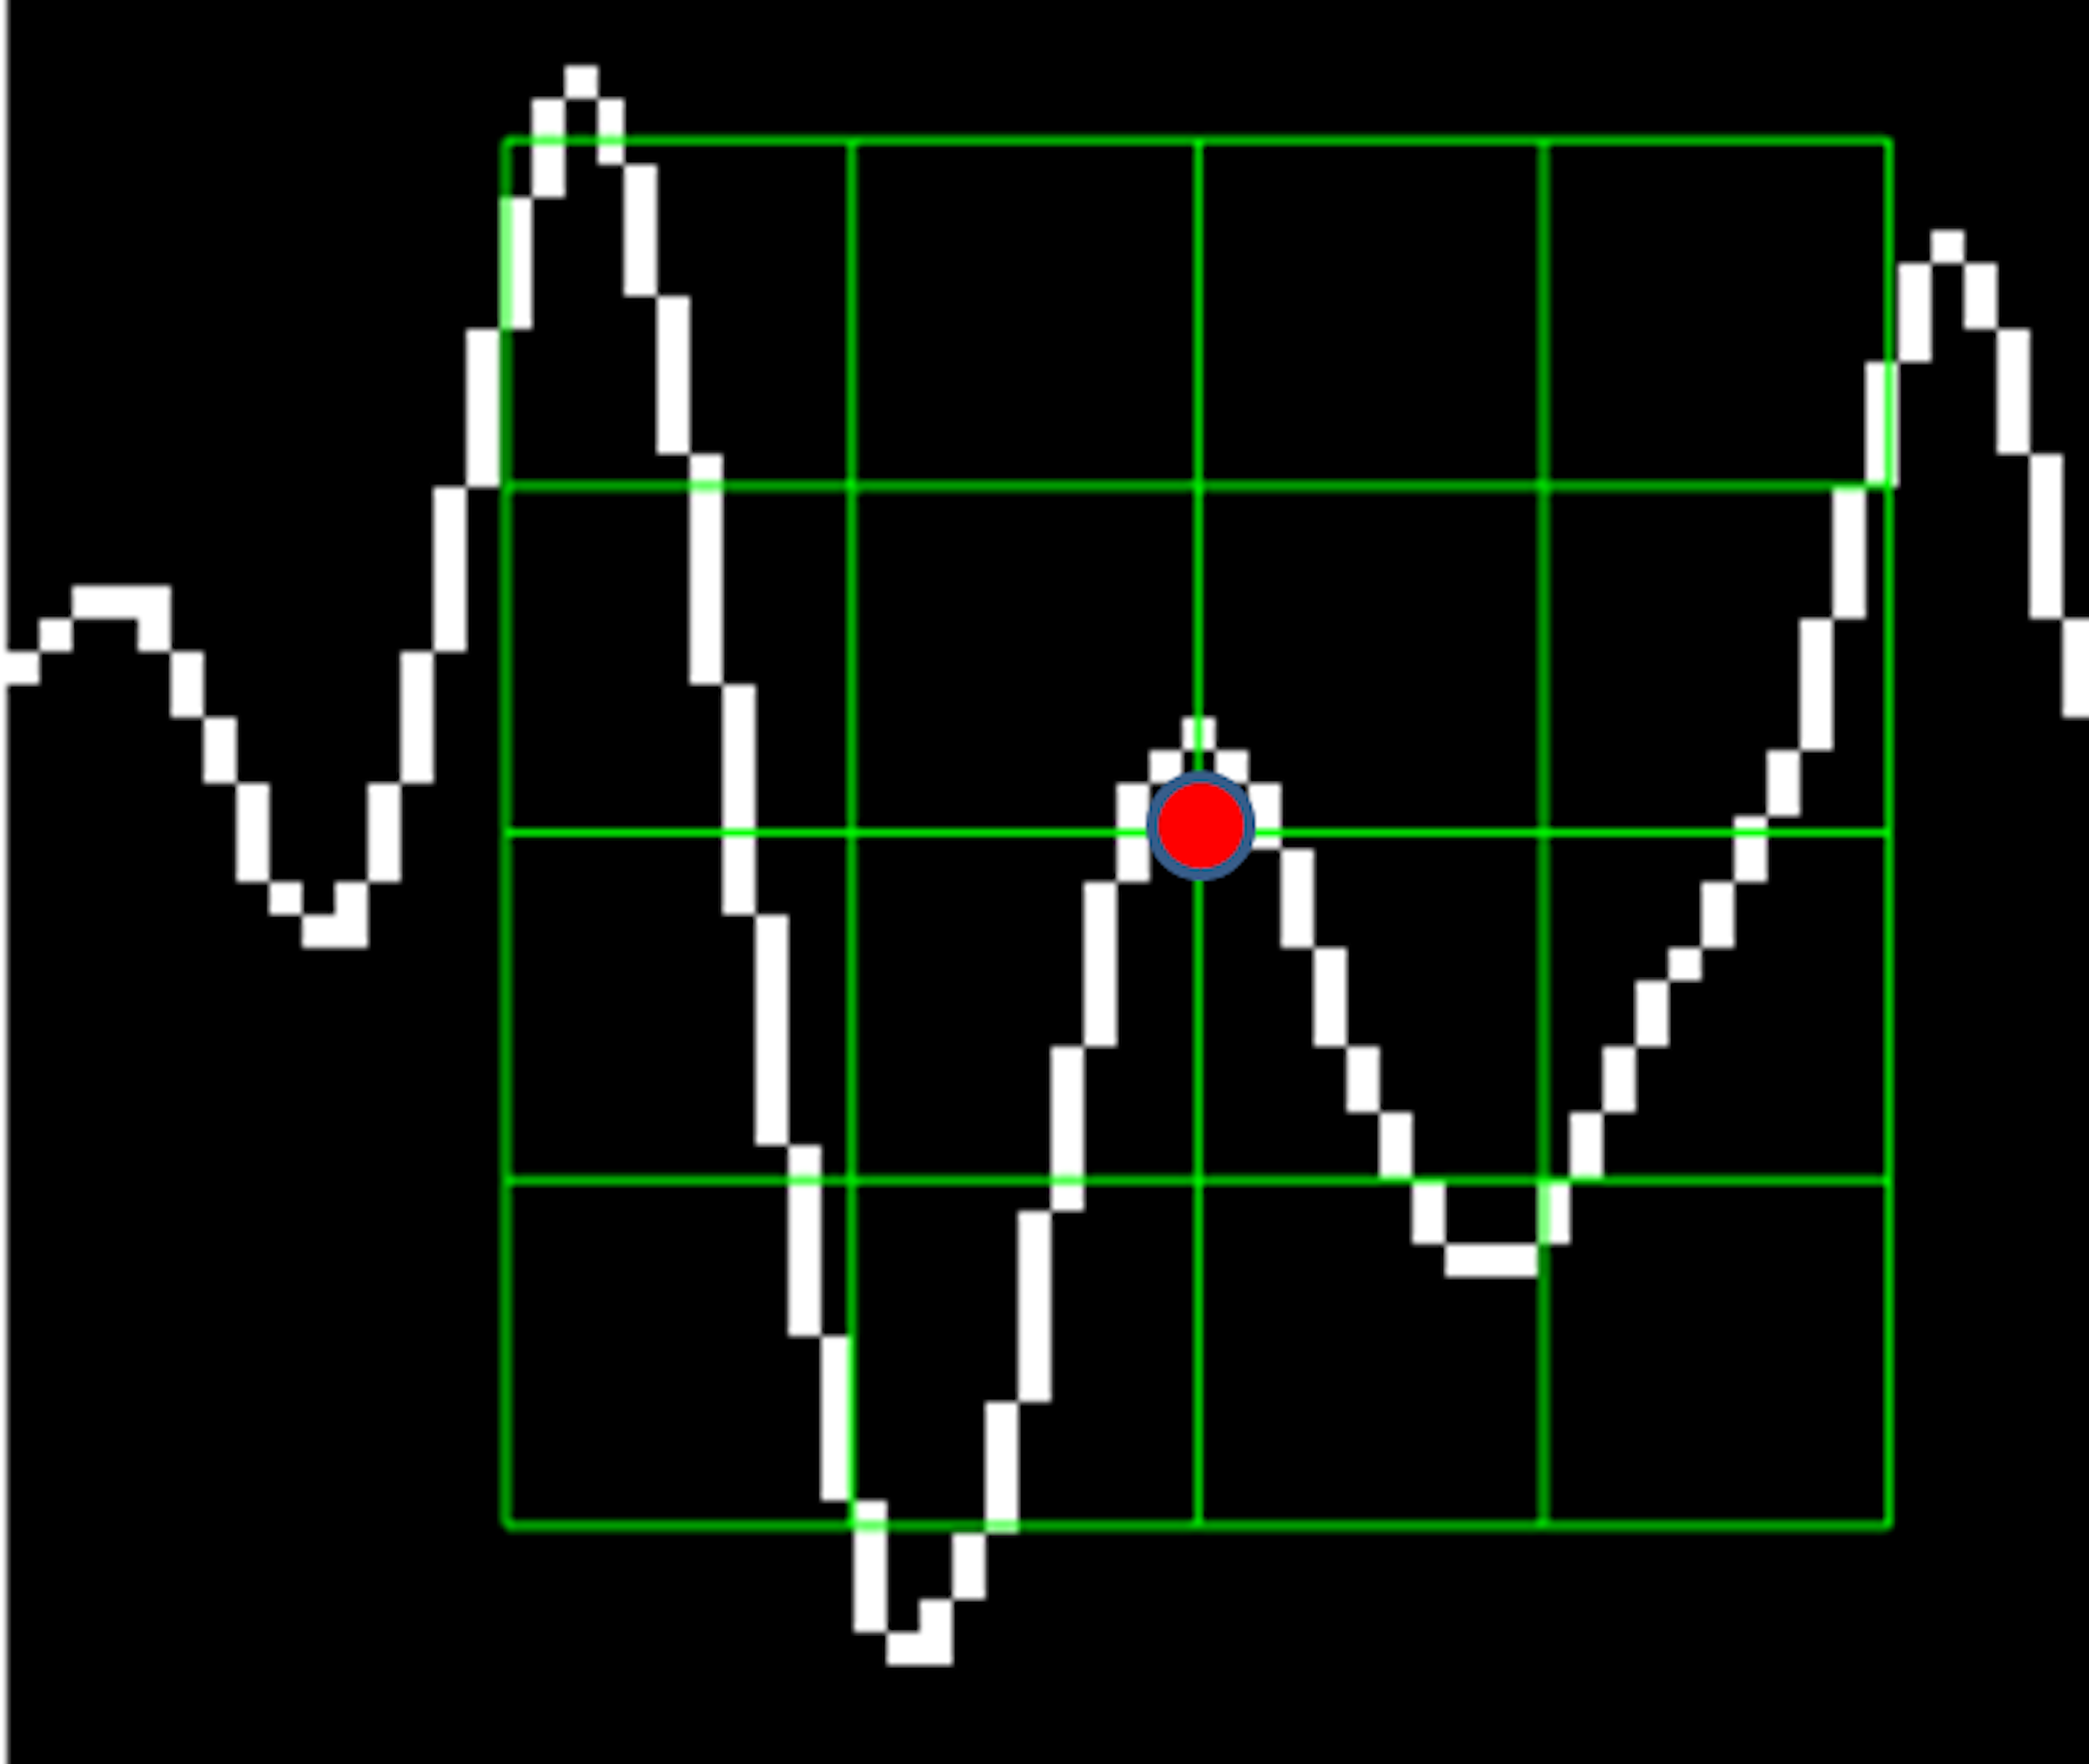
\includegraphics[width=7cm, height=6cm]{images/signalpatchkeypoint.png}}
\subfigure[A Sobel filter is applied to the image and a vector field of oriented gradients is calculated for each pixel.]
{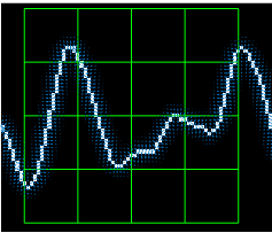
\includegraphics[width=7cm, height=6.1cm]{images/gradientsdescriptors.png}}
\subfigure[Zoomed-in vector field of oriented gradients around the signal plot.  Each pixel is assigned an orientation and magnitude.]
{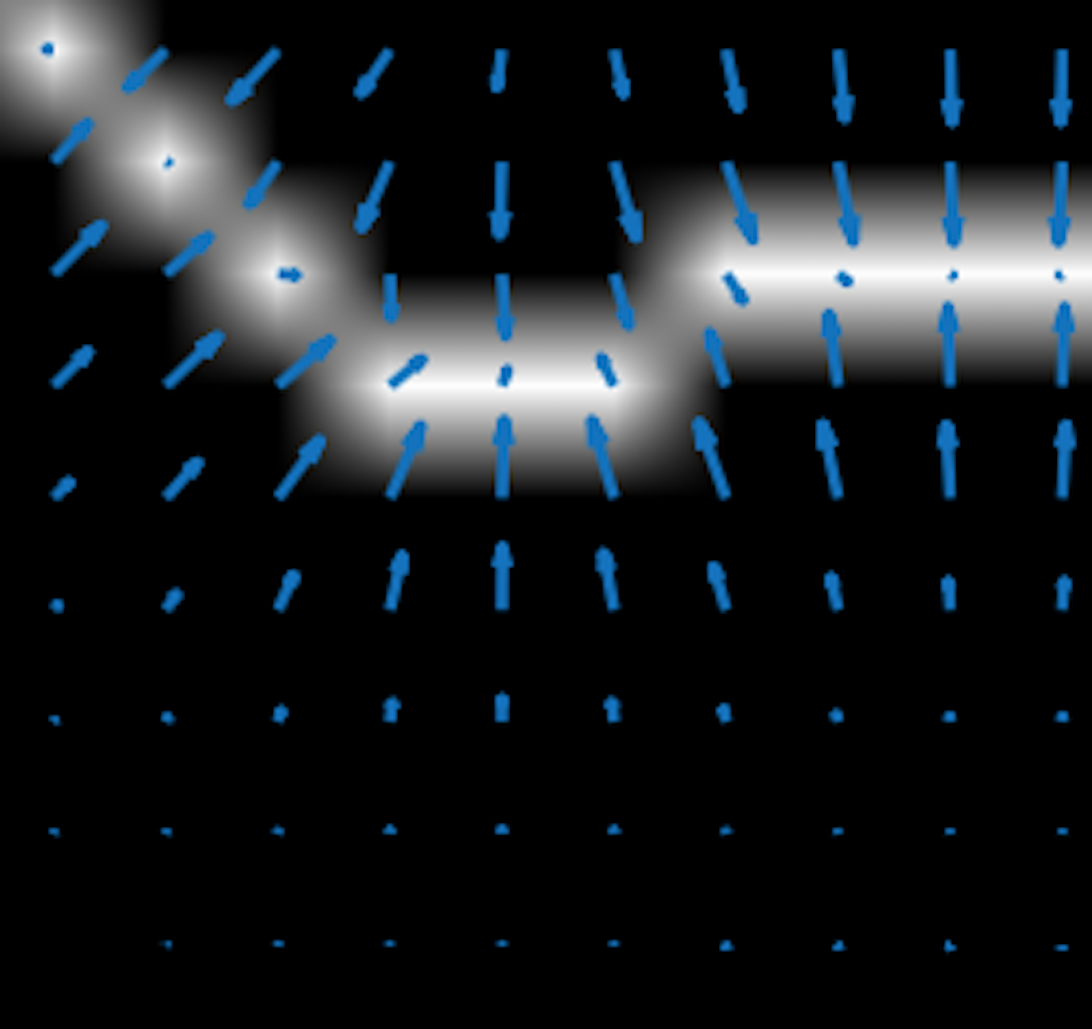
\includegraphics[width=7cm, height=6cm]{images/samplegradients.png}}
\subfigure[Eight oriented bins are used on each block to identify the oriented gradients within each block.]
{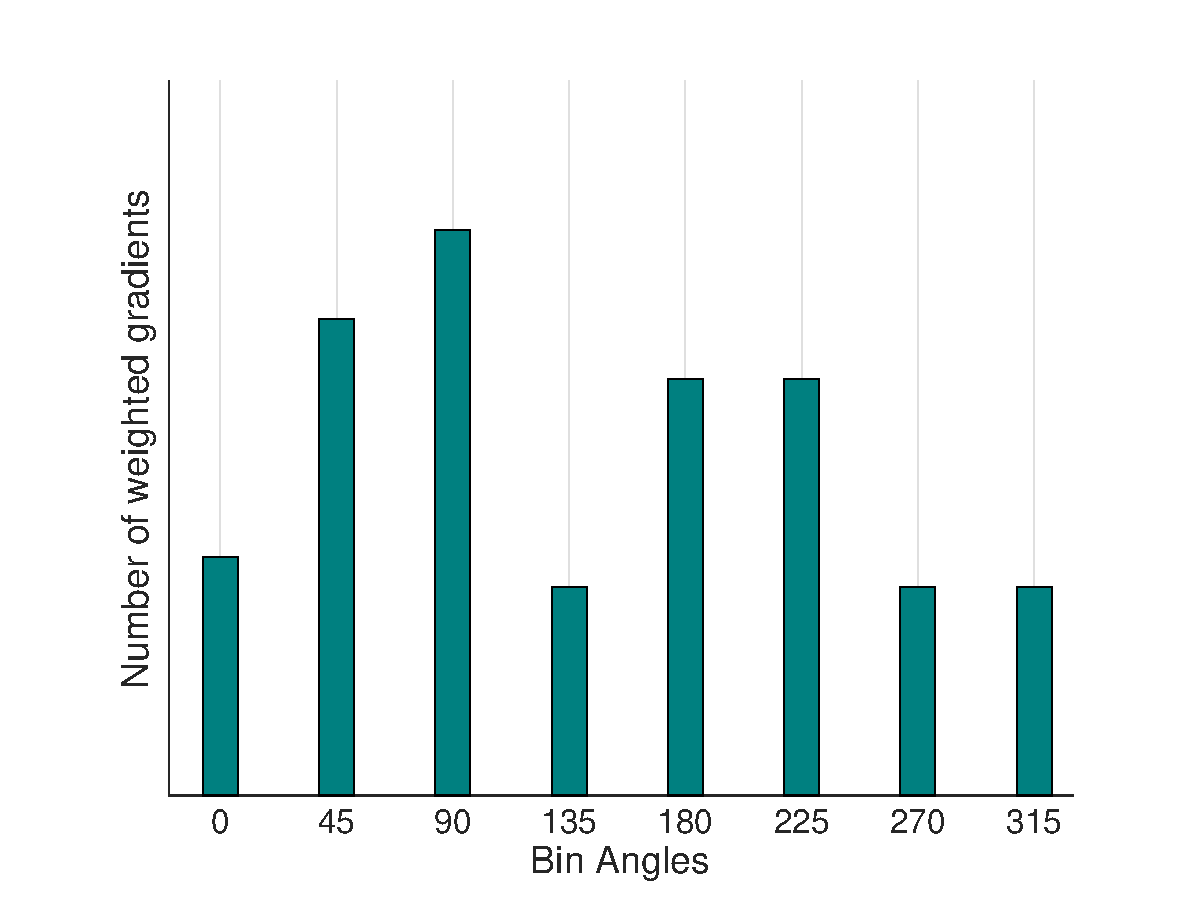
\includegraphics[width=7cm, height=6cm]{images/histogramchart.eps}}
\caption[Histogram of Gradient Orientations]{Patch and vector field of oriented gradients.}.
\label{fig:sampledescriptor}
\end{figure}


\begin{figure}[h!]
\centering
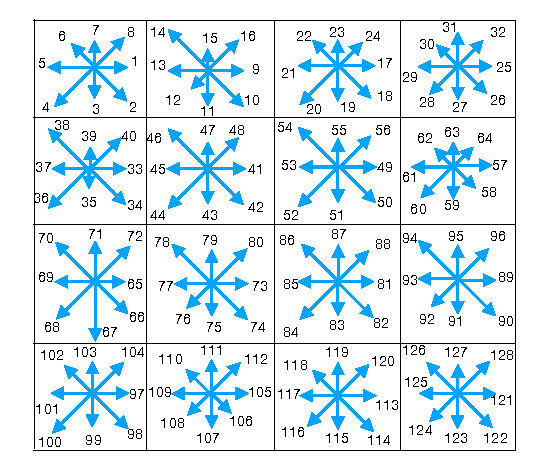
\includegraphics[width=16cm]{images/gradientorientations.pdf}
\caption[Gradient Orientations Numbering]{A scheme of the orientation's histogram computation. The first eight orientations of the first block $ B_{1,1} $, are labeled from $1$ to $8$ clockwise. The orientation of the second block $ B_{1,2} $ is labeled from $9$ to $16$.  This labeling continues left-to-right, up-down until the eight orientations for all the sixteen blocks are assigned. They form the corresponding descriptor of $128$ coordinates.  The length of each arrow represent the value of the histogram on each direction for each block.}
\label{fig:orientationsfull}
\end{figure}


%\begin{figure}[h!]
%\centering
%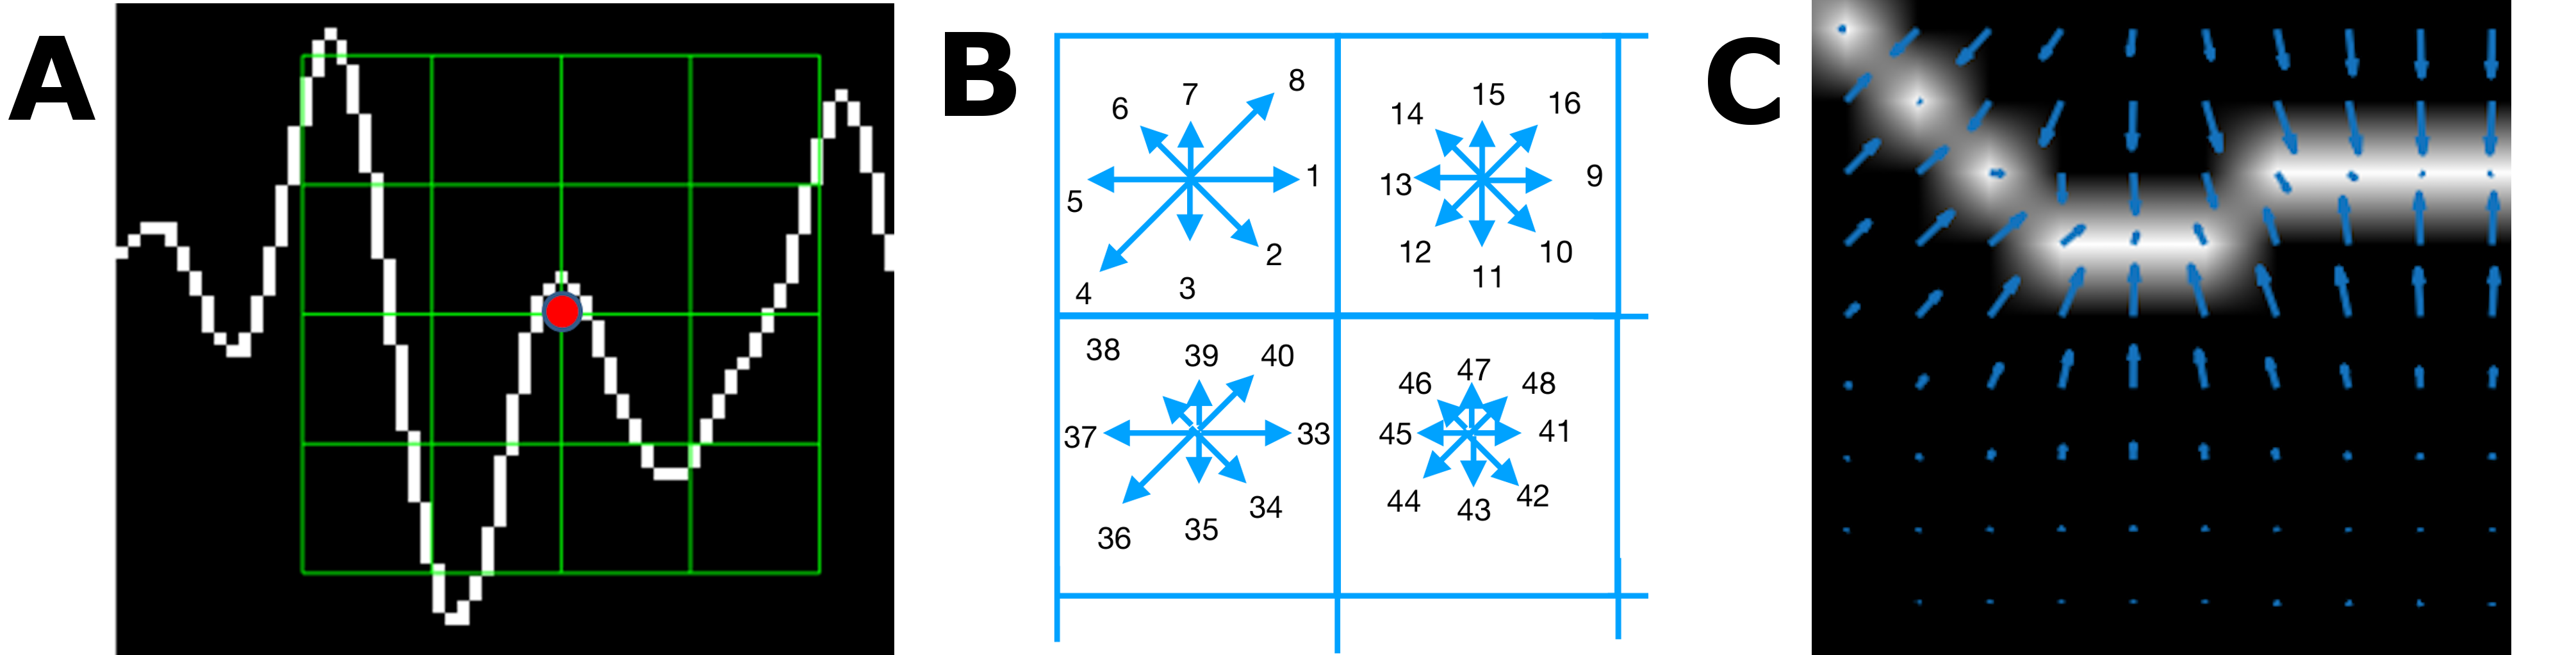
\includegraphics[width=16cm]{images/gradients.png}\label{samplegradients}
%\caption[Histogram of Gradient Orientations for ERP]{ (A) Example of a plot of the signal, a keypoint and the corresponding patch. (B) A scheme of the orientation's histogram computation.  Only the upper-left four blocks are visible.  The first eight orientations of the first block, are labeled from $1$ to $8$ clockwise. The orientation of the second block $ B_{1,2} $ is labeled from $9$ to $16$.  This labeling continues left-to-right, up-down until the eight orientations for all the sixteen blocks are assigned. They form the corresponding descriptor of $128$ coordinates.  The length of each arrow represent the value of the histogram on each direction for each block. (C) Vector field of oriented gradients.  Each pixel is assigned an orientation and magnitude calculated  using finite differences. }
%\label{fig:sampledescriptor}
%\end{figure}

%\begin{figure}[h!]
%\centering
%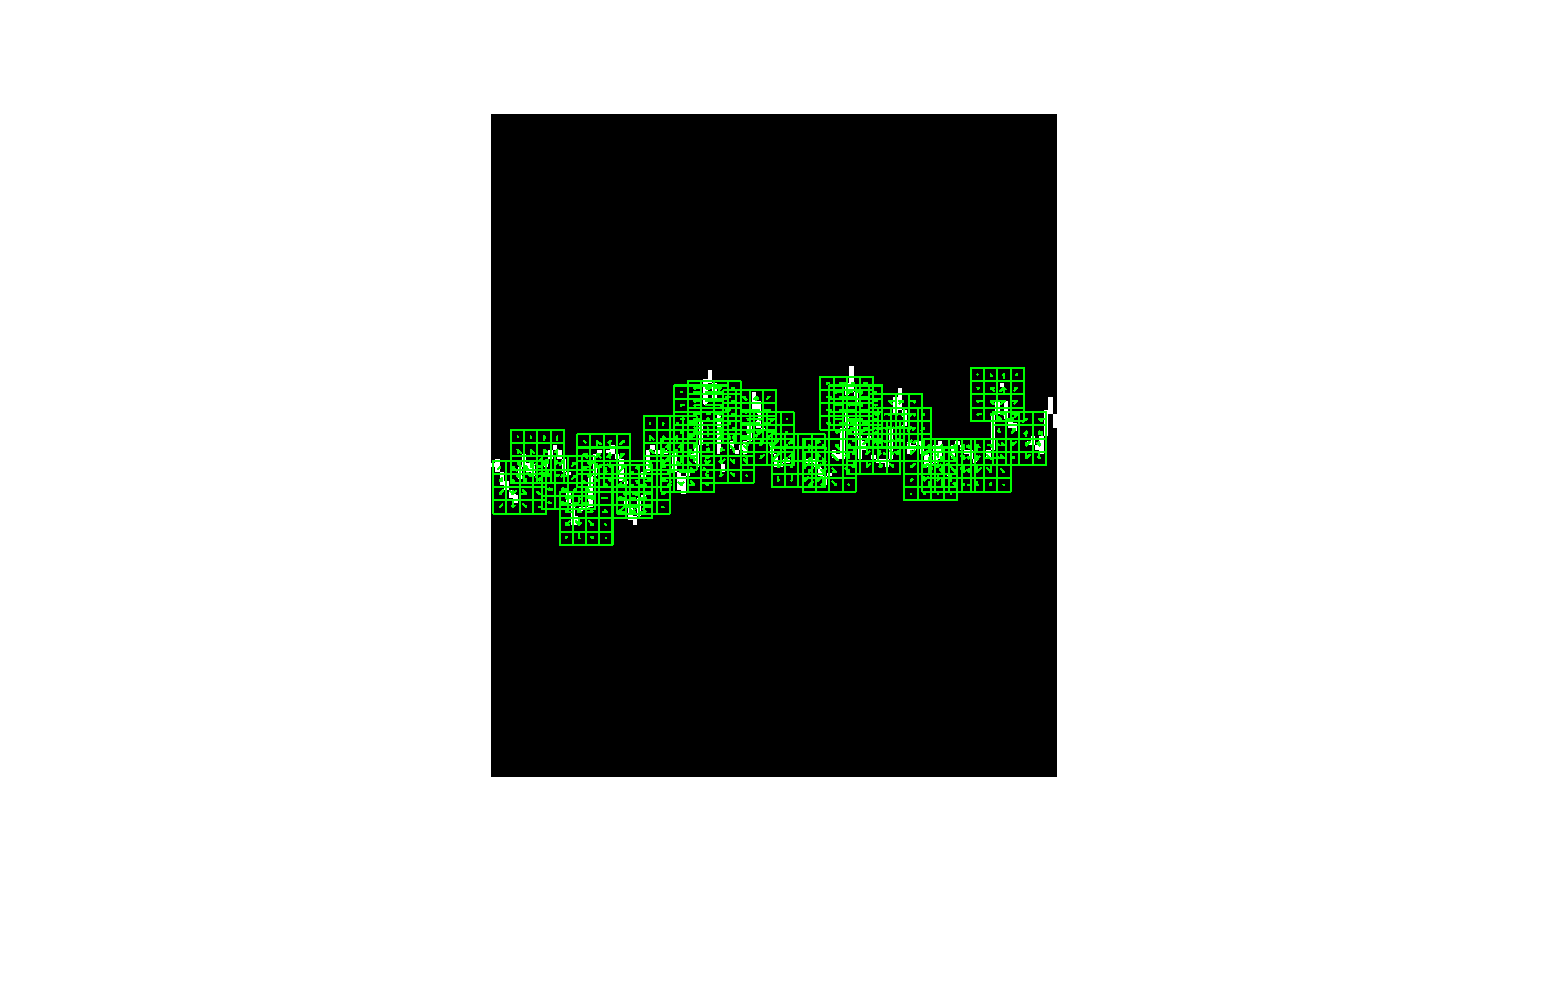
\includegraphics[scale=0.6]{images/KeypointLocations.eps}
%\caption[SIFT Patches]{fdsfdfsfs }
%\label{fig:siftpatch}
%\end{figure}


\section{Keypoint Location}
\label{keypointlocation}

%TODO Vertidal: Along the signal or zero level.
% Horizontal: based on a cognitive event, one or many.
%


The keypoint $\gls{kp}$ location must be accurately specified in order to establish the region from the signal where the waveform is located.

For the horizontal position, the localization of the keypoint is based on a priori information, based on the characteristics of the event under study.  For instance, ERPs have a specific timing that can be explored to elucidate in which position the expected signal pattern will be generated.

Additionally, there can be more than just one keypoint and patch located over the signal plot.  This is particular important for oscillatory processes where many waveforms are contained within the same signal segment.  This needs to be addresses by defining a keypoint density parameter $\gls{kpd}$.  A value of $\gls{kpd}=1$ determines that keypoint are located on every sample point that is used to mark a pixel en Equation~\ref{eq:images}.  A value of $\gls{kpd}=2$ implies that keypoints are located after two sample points, and so on.  Figure~\ref{fig:keypointlocations}(a) shows keypoints being located at a keypoint density $\gls{kpd}$ equals to $10$.

\begin{figure}[h!]
\centering
\subfigure[Fixed size patches are located all along the EEG signal trace at a given keypoint density $\gls{kpd}$. Closed to image's margins no keypoint are located.]
{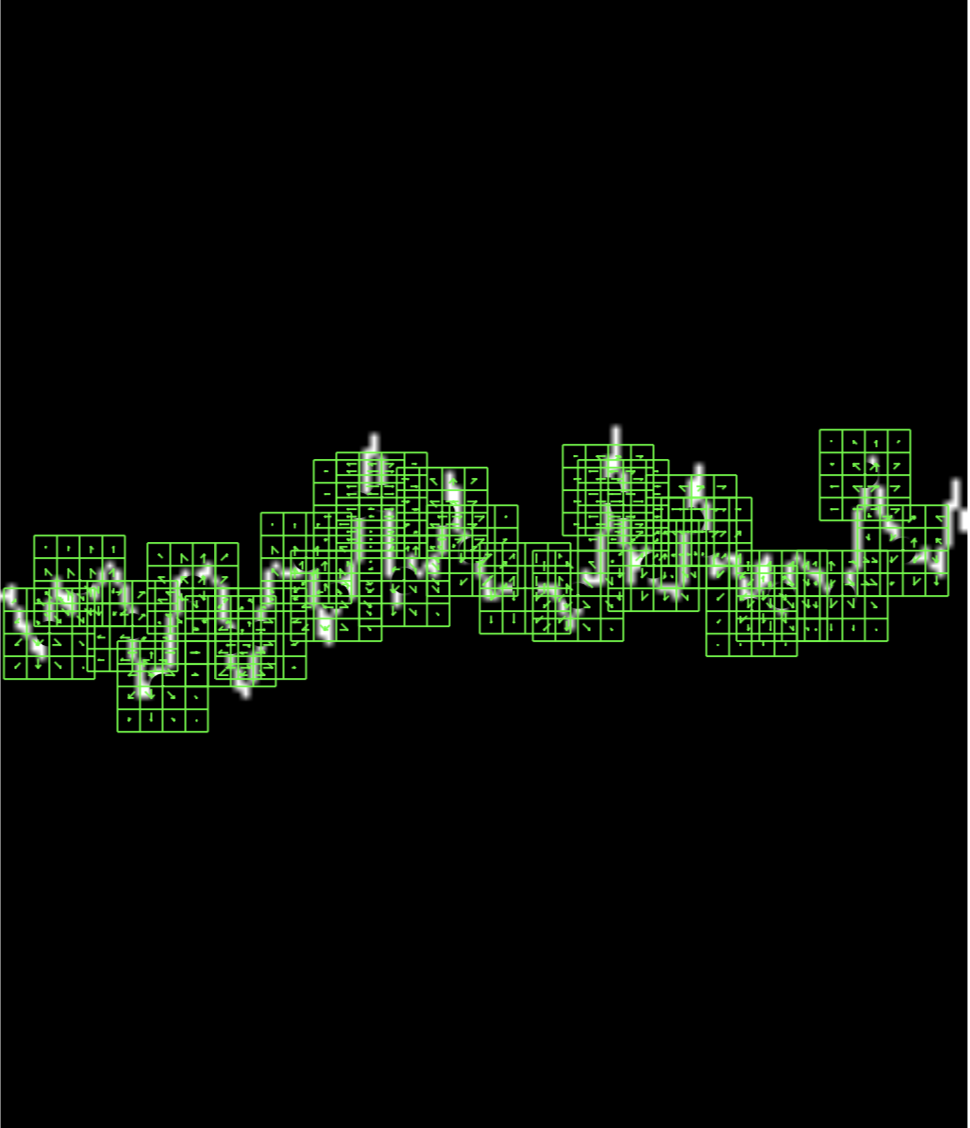
\includegraphics[width=7.5cm, height=7cm]{images/SignalWithFullDescriptors3.png}}
\subfigure[A patch is used to map an artificial signal using an autoscale plotting scheme, and mapping the entire waveform within the patch. The keypoint is located on the zero-level $z(c)$ value.]
{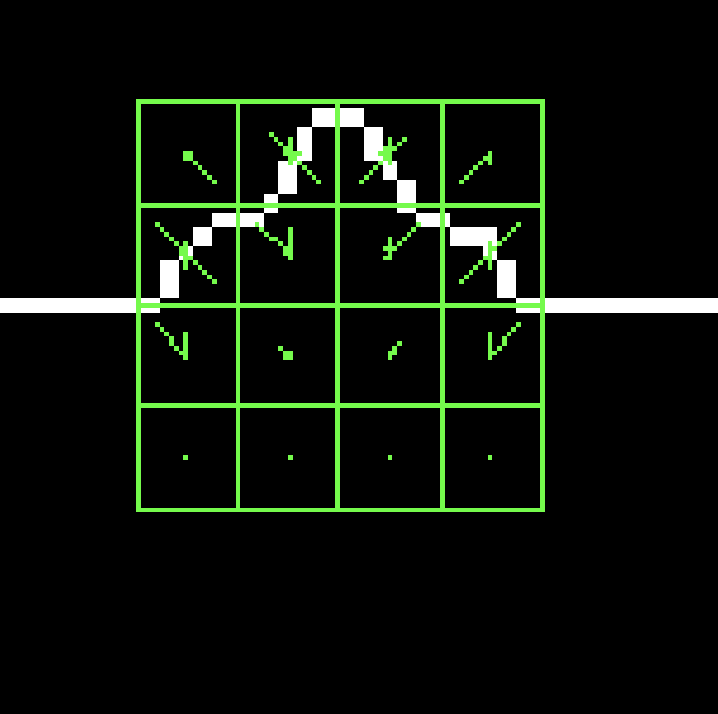
\includegraphics[width=7.5cm, height=7cm]{images/EasyDescriptorSample3.png}}
%\subfigure[Only one fixed size patches are used on a very specific position of the signal trace.]
%{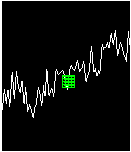
\includegraphics[width=6cm, height=6cm]{images/SignalWithDescriptorSample1.png}}
%\subfigure[An entire signal is mapped with fixed size patches with a very high keypoint density $\gls{kpd}$.]
%{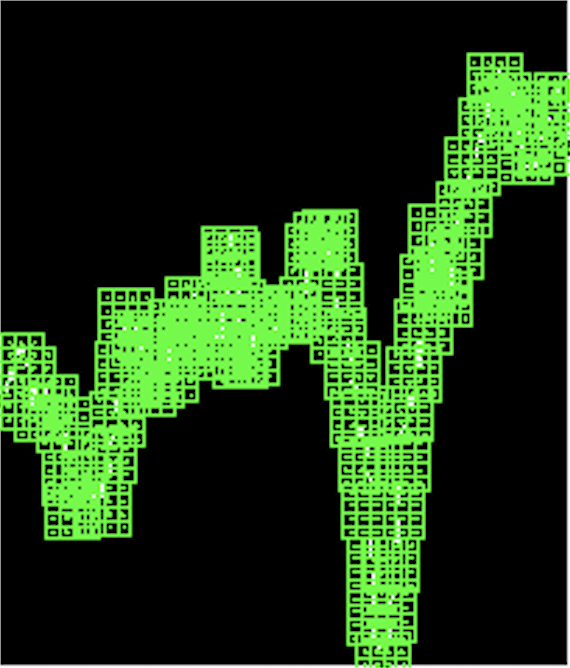
\includegraphics[width=6cm, height=6cm]{images/SignalWithFullDescriptors2.png}}
\caption[Keypoint Locations]{Two different alternatives of keypoint locations and patch geometry.}.
\label{fig:keypointlocations}
\end{figure}

%TODO en realidad son tres, en el zero level a la mitad de la imagen o en el eeg trace.

Regarding the Vertical Location, there are two options.  The first one is along the signal, exactly on the sample points calculated by the Equation \ref{eq:images}.  The second is on a fixed position over the zero-level as described by \ref{eq:zerolevel}.  Figure~\ref{fig:keypointlocations}(a) show the former while on~\ref{fig:keypointlocations}(b) the latter can be spotted.

\section{Patch Geometry}
\label{patchgeometry}

%TODO Vertical size: Fixed for autoscaled and variable.
% Horizontal: based on a priori information

The standard implementation of the SIFT Descriptor uses a squared-size patch, and there is only one scale parameter $S$.  However, this is not appropriate to capture waveforms which may expand on the horizontal axis, on the time scale.  The Histogram of Gradient Orientations on the other hand, allows to have a rectangular patch geometry which can be used to cover an entire waveform, regardless of their span $\gls{lambda}$.  The original SIFT scale, is modified in this implementation to allow two scale parameters, one per each axis.

The Horizontal Patch Scale $\gls{St}$ determines the size of the patch on the image horizontal axis, and it is related to the span $\gls{lambda}$ of the waveform to analyze according to

\begin{equation}
\gls{St} = \frac{ \gls{lambda} \;  \  \gls{Fs} \ \gls{gammat} }{\gls{Deltas}}
\label{eq:horizontalpatchscale}
\end{equation}

\noindent where $\gls{Fs}$ is the sample frequency, $\gls{gammat}$ is the time scale factor and $\gls{Deltas}$ is the unit length of the patch which determines the pixel conversion factor.  This value depends on the actual implementation of the Histogram of Gradient Orientations of the SIFT method. In this case, its value is $\gls{Deltas} = \sqrt{2} \; 3 \; 5$, where $3$ is the fixed magnification factor, and $5$ correspond to the number of blocks in which the patch is divided, plus half the size of the block on each direction.  Check Appendix~\ref{chapter:eleven} for details on the SIFT method implementation.

On the other hand, on the vertical axis, the vertical patch scale depends on the peak-to-peak amplitude $\gls{DeltamuV}$, and the amplitude scale factor $\gls{gamma}$, as

\begin{equation}
\gls{Sv} = \frac{\gls{DeltamuV} \ \gls{gamma}}{\gls{Deltas}}.
\label{eq:verticalpatchscale}
\end{equation}

The vertical scale can be dynamically adjusted according to the peak-to-peak amplitude of each segment, or it can be set fixed.  This is more appropiate if the underlying signal is bounded which is the case if the standardized procedure described in \ref{standardized} is applied.

\begin{figure}[h!]
\centering
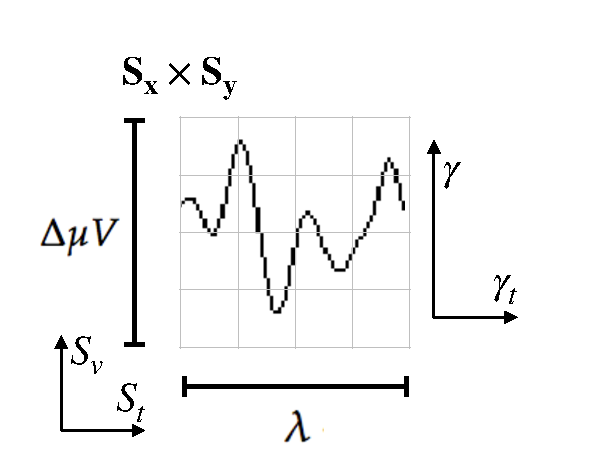
\includegraphics[width=10cm]{images/patchgeometry.pdf}
\caption[Patch Geometry]{The scale of local patch is selected in order to capture the whole waveform, which can be scaled in the time $\gls{gammat}$ and amplitude $\gls{gamma}$ direction.  This determines appropriate horizontal $\gls{St}$ and vertical $\gls{Sv}$ patch scales.  The size of the patch is $\gls{Sx} \times \gls{Sy}$ pixels. The vertical size consists of $4$ blocks of size $\gls{Sy}$ pixels which should be high enough as to contain the signal $\gls{DeltamuV}$, the peak-to-peak amplitude of the signal component. The horizontal size includes $4$ blocks, up to $\gls{Sx}$ pixels, and should cover the entire duration in seconds of the signal waveform, $\gls{lambda}$.   }
\label{fig:patchgeometry}
\end{figure}

Figure~\ref{fig:patchgeometry} shows the different parameters of the patch and how they are related to the underlying signal. Once these parameters are set, the size in pixels of the patch can be obtained in both dimensions.  Hence, the horizontal patch size in pixels is

\begin{equation}
\gls{Sx} = \lfloor \gls{Deltas} \; \gls{St} \rfloor + 1
\label{eq:sx}
\end{equation}

\noindent and the vertical patch size in pixels can be calculated from

\begin{equation}
\gls{Sy} = \lfloor \gls{Deltas} \; \gls{Sv} \rfloor + 1
\label{eq:sy}
\end{equation}

\noindent where $\gls{Deltas}$ being the unit length of the patch. The parameters $\gls{St}$  and $\gls{Sv}$ are the horizontal and vertical patch scale. This region is arranged in a $4 \times 4$ grid and the pixel $\gls{kp}$ is the patch center.   For instance, for a given set of values of $\gls{Sv} = 1$ and $\gls{St} = 1$, the patch is a squared region on the image of size $22$ pixels.

The patch size cannot be bigger than the image itself, whose width is $\gls{Wx}$ and its height is $\gls{Hy}$ .  This is reflected by the following two inequalities that restrict the size of the patch according to 

\begin{equation}
\frac{\gls{Wx}-1}{\gls{Deltas}}  \geq \gls{St} ,
\label{eq:restriction1}
\end{equation}

\noindent on the horizontal axis, and on the vertical axis, 

\begin{equation}
\frac{\gls{Hy}-1}{\gls{Deltas}}  \geq \gls{Sv}.
\label{eq:restriction2}
\end{equation}

\subsection{Oscillatory Processes}

For these patterns, the strategy is to locate keypoints, and their patches, all along the signal trace, filling the entire signal segments with all the possible patches.  In this case, the keypoint density $\gls{kpd} $ determines the step at which a keypoint is located along the trace of the signal, sample point after sample point. Care must be taken close to the margins, where there should be a gap to avoid locating incomplete patches.  This can be observed in Figure~\ref{fig:keypointlocations}(a).

\subsection{Transient Events}

For transient events, descriptors are treated as representatives of the single transient waveforms.  This leads to usually just one keypoint that is located in a meaningful position along the horizontal axis.  Additionally, for autoscale plotting, the zero level can be used to localize keypoints. Figure~\ref{fig:keypointlocations}(b) shows the plot of an artificial waveform with the corresponding patch.

\section{BCI Algorithm}

Now that all the ingredients have been exposed, the general layout of the BCI algorithm can be described.  Going back to BCI model referenced in~\ref{fig:bciblockdiagram}, the following sections outline the Preprocessing, Calibration and Classification step.

\begin{story}[Terminology Clarification]
\theoremstyle{definition}

\begin{definition}{Keypoint:}
\label{def:Keypoint}
\textit{A keypoint is a specific pixel on the image.  The keypoint is the center of a patch and it is used to outline a region of interest.}
\end{definition}

\begin{definition}{Patch:}
\label{def:Patch}
\textit{An image region centered around a keypoint.  It is divided in a rectangular 4x4 grid.}
\end{definition}

\begin{definition}{Descriptor:}
\label{def:Descriptor}
\textit{A 128-dimensional \textit{feature} vector.  Contains the histogram of 8 angular directions per each block of the 16 blocks of the patch.}
\end{definition}

\begin{definition}{Waveform:}
\label{def:Waveform}
\textit{A signal shape, a transient component or an oscillatory wave, with a potential cognitive implication.}
\end{definition}

\begin{definition}{Signal:}
\label{def:Signal}
\textit{The EEG Signal. This Thesis refers to a multidimensional signal or to a single-channel signal. When the clarification is of relevance, it is provided.}
\end{definition}

\begin{definition}{Image:}
\label{def:Image}
\textit{The \textit{canvas} with sample points created from equation~\ref{eq:images}.}
\end{definition}

\begin{definition}{Plot:}
\label{def:Plot}
\textit{The trace of the EEG signal on the Image.}
\end{definition}

\begin{definition}{HIST:}
\label{def:Plot}
\textit{This the acronym that hereafter is being used to describe the feature extraction method proposed in this Thesis.}
\end{definition}

\end{story}

\subsection{Preprocessing}

Signal preprocessing can be applied to $x(n,c)$ before applying the plotting scheme.  Preprocessing depends on the cognitive paradigm under study.  

%TODO completar esto
%\begin{itemize}
%\item Notch filter:
%\item Band-pass filter
%\item Decimation or Downsizing:
%\item Segmentation
%\item Baseline Removal
%\item Artifact Rejection
%\item Spatial Filter
%\end{itemize}
%
%An excellent review can be found here~\cite{Simons2016}.

\subsection{Calibration}
\label{Calibration}

The calibration step of BCI entails designing an experimental protocol or procedure to allow the computer to learn the signals that identify a cognitive pattern.  Once those patterns are learned, the BCI system tries to identify new unlabeled signals comparing them against those learned patterns.  By performing the feature extraction method outlined in this Chapter, descriptors can be extracted from images and stored in template dictionaries.  These templates are generated on a channel-by-channel basis.  Each dictionary $T^{bpc}$ is used to represent one type of signal to discriminate. The data structure proposed to store descriptors is a KD-tree~\cite{Lowe2004}.

Moreover, the calibration can be also used to identify the $\gls{bpc}$, the Best Performing Channel. This value is used to evaluate the spatial performance based on the electrode where the best classification accuracy is obtained~\cite{Chavarriaga2017}.

\subsection{Classification}
\label{nbnn}

A discriminative~\cite{WolpawJonathanR2012} semi-supervised classification method based on Naive Bayes Nearest Neighbor (NBNN)~\cite{Boiman2008} is applied to classify EEG signals using the features provided by the calculated descriptors. In order to classify a new image, a query image, $Q$ descriptors are extracted from it.  The NBNN technique allows to categorize this image to one class by comparing the set of extracted descriptors $\mathbf{q}_{i}^{(bpc)}$ to those which are more similar on each dictionary $T^{bpc}$.  This algorithm is very easy to implement, and is based on the following Equation:

\begin{equation}
\hat{L} = \arg \min_{L} \sum_{i=1}^{Q} \sum_{h=1}^{\gls{k}} {\left\lVert \mathbf{q}_{i}^{(bpc)} -  \mathbf{d}_{h}^{(bpc)} \right\rVert}  ^{2} 
\label{eq:classification}
\end{equation}

\noindent where the $Q$ descriptors $ \mathbf{q}_{i}^{(bpc)} $ are extracted from a query image for the $\gls{bpc}$ and, the dictionary descriptors  $\mathbf{d}_{h}^{(bpc)} \in N_T(  \mathbf{q}_{i}^{(bpc)} )$ with the set $N_T(  \mathbf{q}_{i}^{(bpc)} ) $ defined as $N_T(  \mathbf{q}_{i}^{(bpc)} ) = \{ \mathbf{d}_{h}^{(bpc)} \in T_{L}^{bpc} / \mathbf{d} $ is the $\gls{k}$-nearest neighbor of $  \mathbf{q}_{i}^{(bpc)} \}$.  This set is obtained by sorting all the elements $ \mathbf{d}_{h}^{(bpc)} $ in $T_{L}^{bpc}$ based on distances between them and $\mathbf{q}_{i}^{(bpc)}$, choosing the $\gls{k}$ with smaller values.  Hence, the estimated class label $\hat{L}$ of a query image is calculated as the class label $L$ that minimizes the summation of the distances between descriptors $\mathbf{q}_{i}^{(bpc)}$ that belong to the query image and their corresponding near neighbor descriptors $\mathbf{d}_{h}^{(bpc)} $  that belong to the template dictionary for each class. Figure~\ref{fig:nbnnclassification} show a scheme of how this classification method works.

\begin{figure}[h!]
\centering
\subfigure[]
{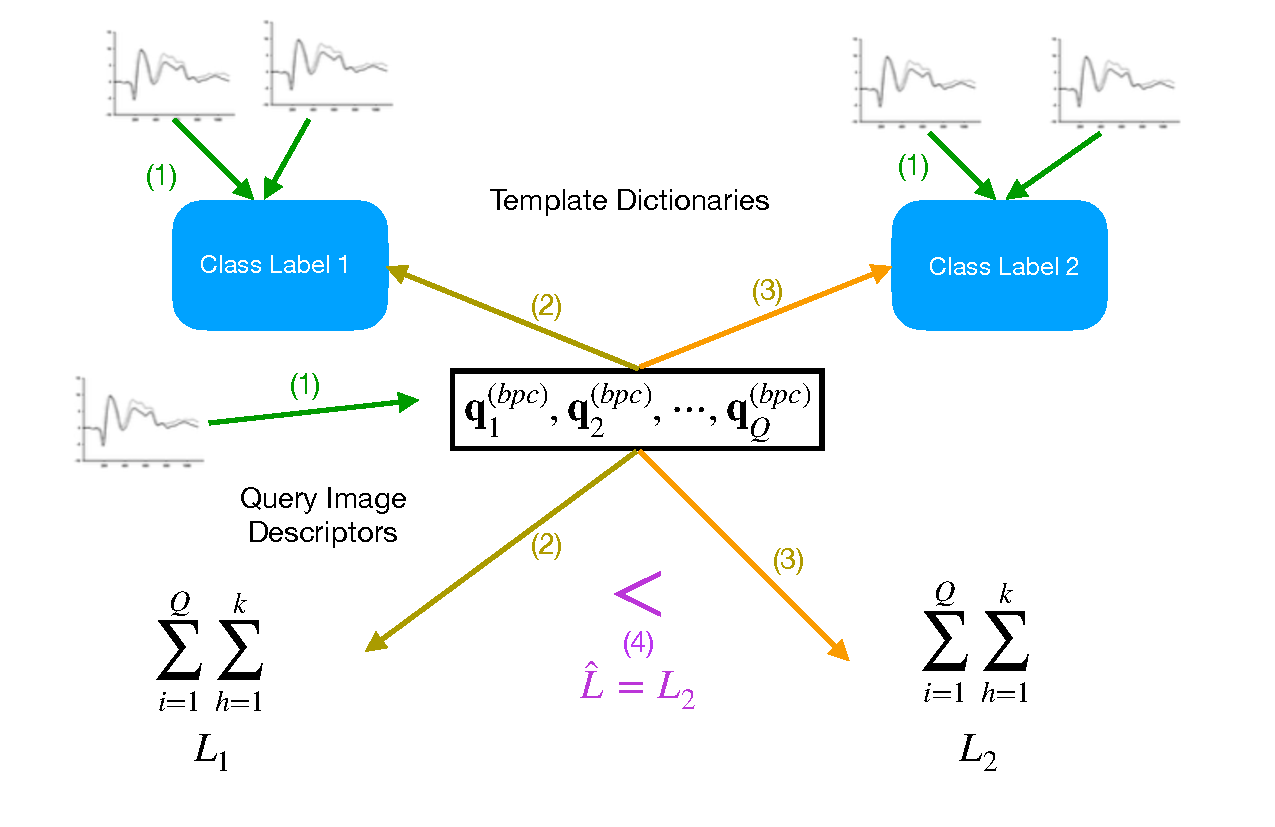
\includegraphics[scale=0.7]{images/ClassificationFull.pdf}}
\caption[NBNN Classification]{Classification Algorithm: \textbf{Step 1} Two Dictionaries are created from templates descriptors obtained in a calibration session for two different classes, labeled $1$ and $2$. On the other hand, a set of query descriptors are extracted from a new image that needs to be categorized. \textbf{Step 2} Distances from every descriptor $q_i$ are calculated against the closest one from the dictionary of class 1.  Distances summations are accumulated. \textbf{Step 3} Distance values from every descriptor $q_i$ are calculated against the closest one from the dictionary of class 2, the other class.  Distances summations are accumulated. \textbf{Step 4 }The two summation values for each class label are compared against each other. The summation that achieved the lesser value is the one that more closely resembles the set of templates, thus is the one predicted by the classification algorithm.}
\label{fig:nbnnclassification}
\end{figure}

%\begin{figure}[h!]
%\centering
%\subfigure[Two Dictionaries contain templates descriptors for two different classes. A set of query descriptors are extracted from a new image that needs to be categorized. ]
%{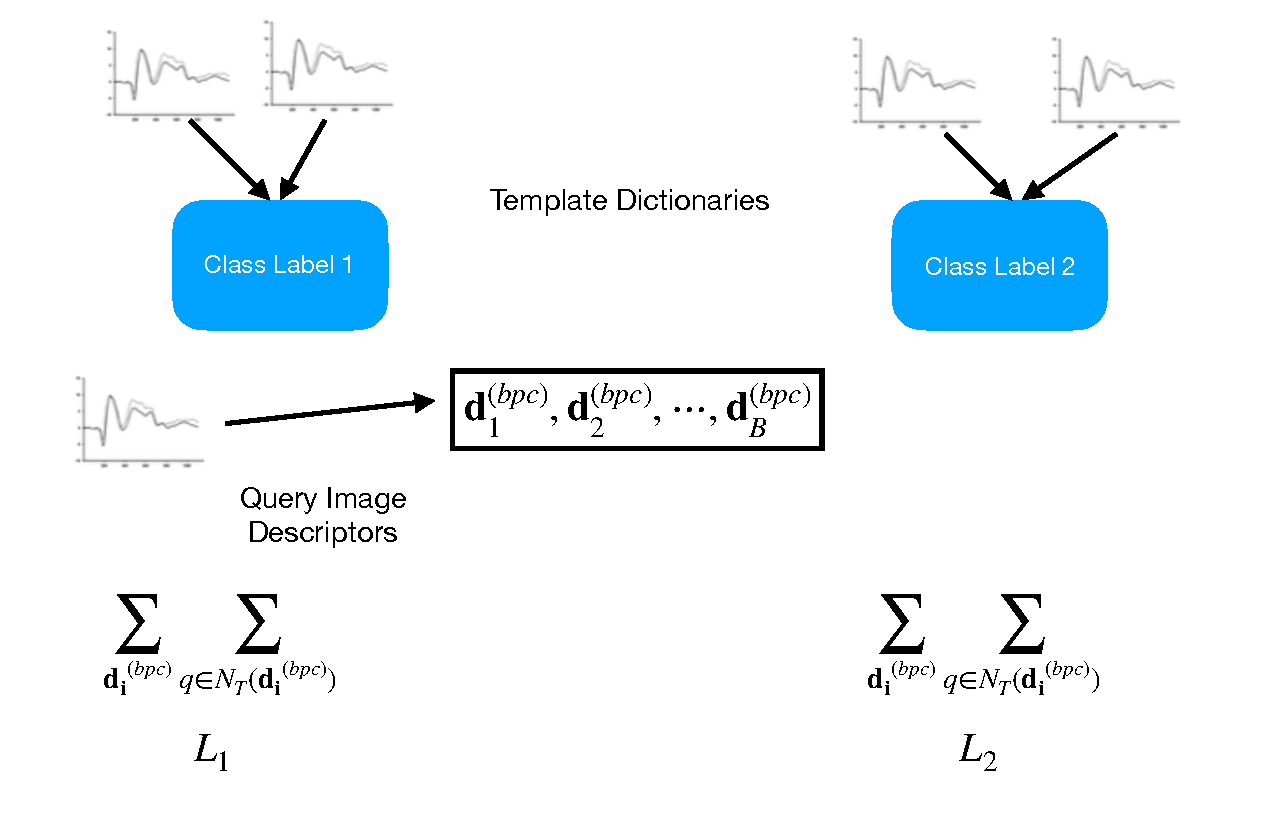
\includegraphics[scale=0.7]{images/Classification1.pdf}}
%\subfigure[Distances from every descriptor $\gls{d}_i$ are calculated against the closest one from the Dictionary of Class 2.  Distances summations are accumulated.]
%{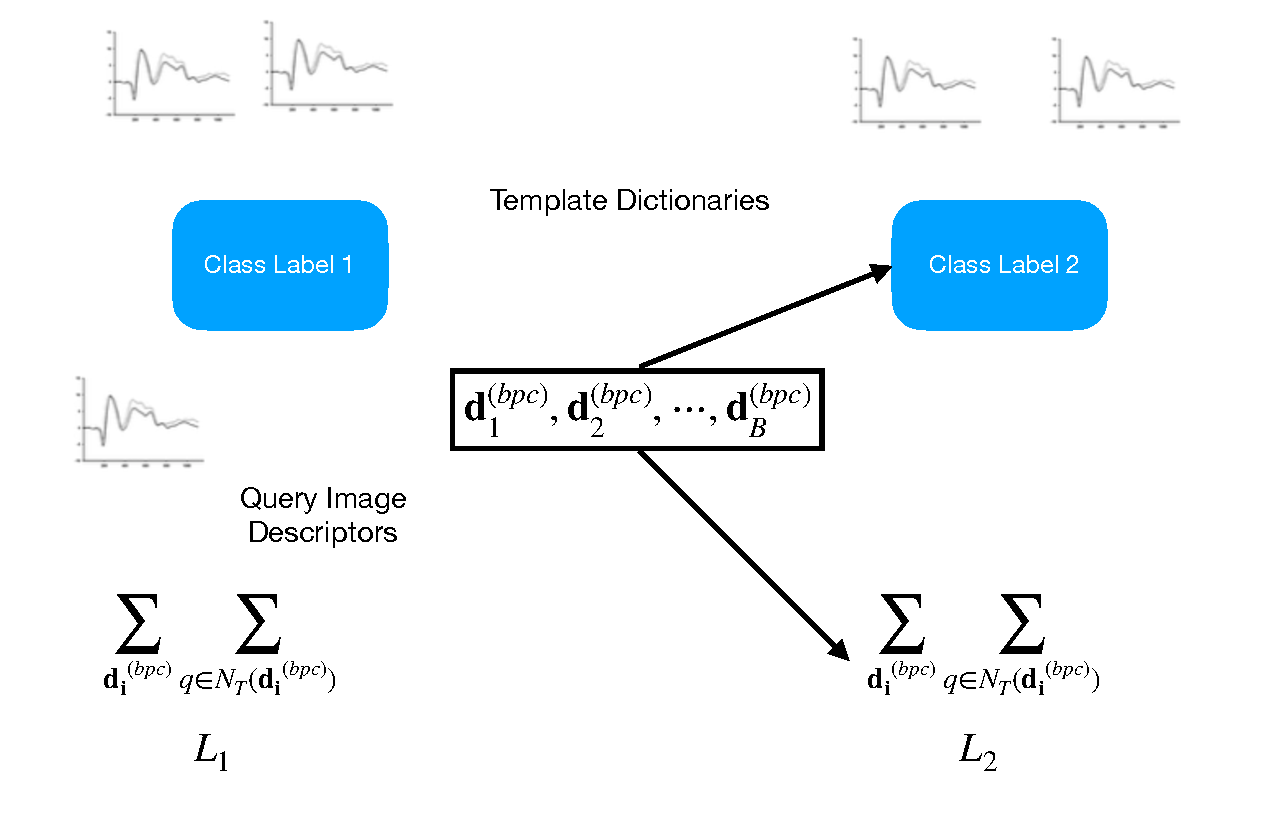
\includegraphics[scale=0.7]{images/Classification2.pdf}}
%\caption[NBNN Classification]{NBNN Classification Scheme}
%\label{fig:nbnnclassification1}
%\end{figure}
%
%\begin{figure}[h!]
%\centering
%\subfigure[Distance values from every descriptor $\gls{d}_i$ are calculated against the closest one from the Dictionary of Class 1.  Distances summations are accumulated. ]
%{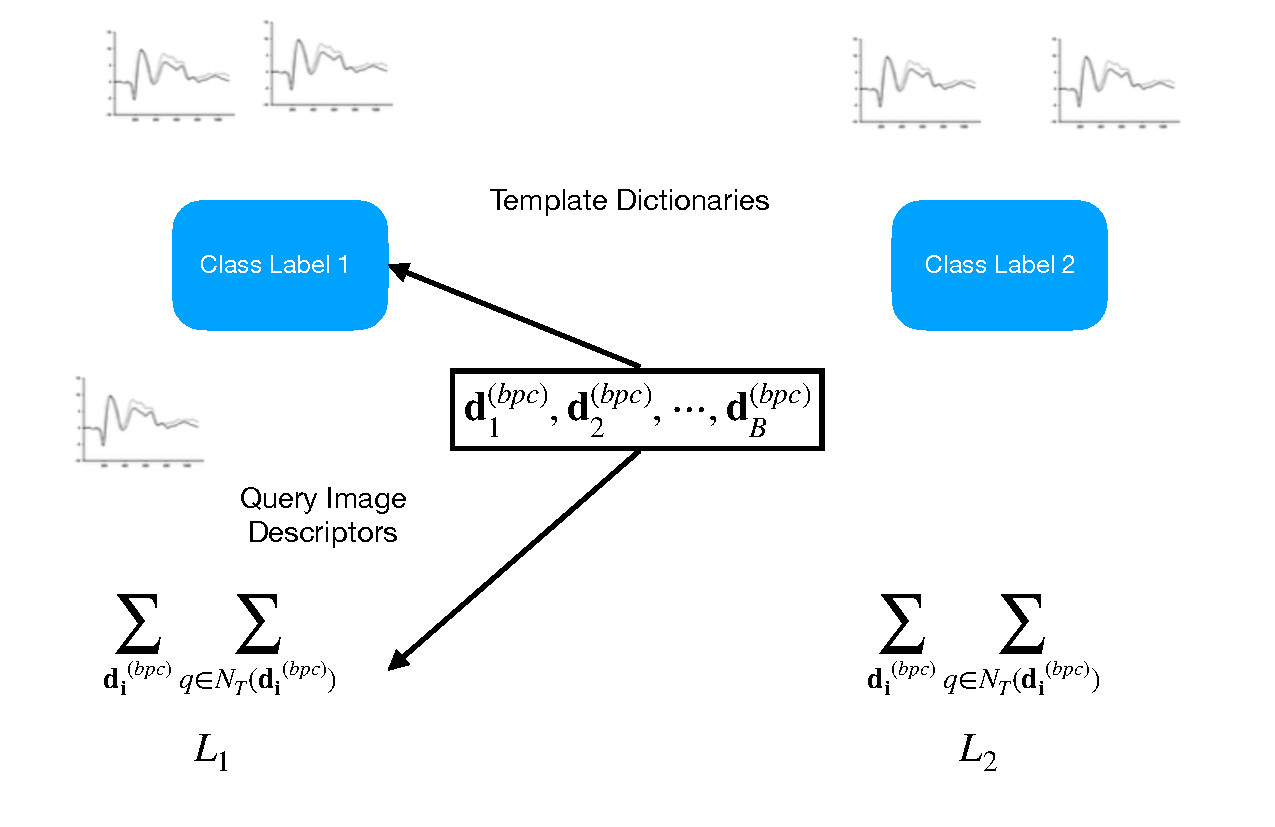
\includegraphics[scale=0.7]{images/Classification3.pdf}}
%\subfigure[The two different summation values are compared against each other. The summation that achieved the lesser value is the one that more closely resembles the set of templates, thus is the one predicted by the classification algorithm.]
%{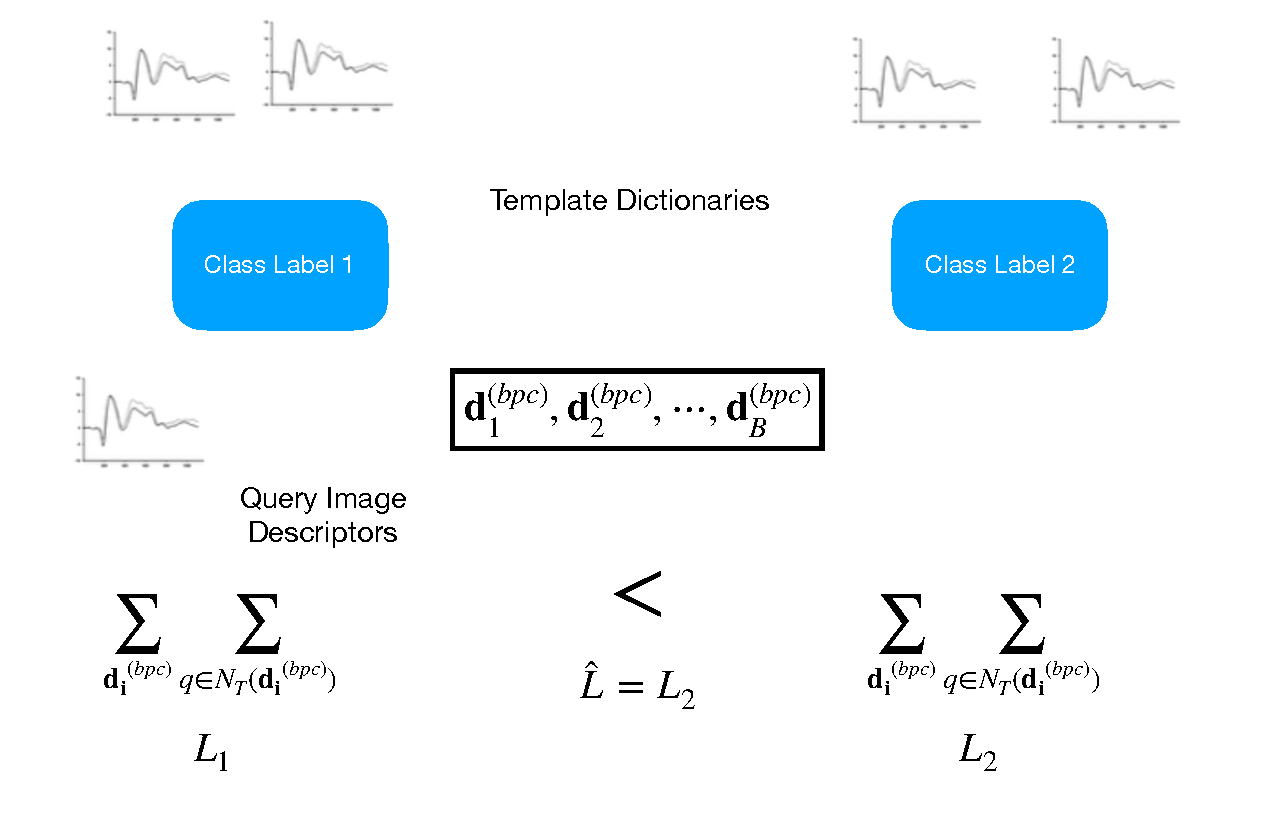
\includegraphics[scale=0.7]{images/Classification4.pdf}}
%\caption[NBNN Classification]{NBNN Classification Scheme}
%\label{fig:nbnnclassification2}
%\end{figure}


%\begin{figure}[h!]
%\centering
%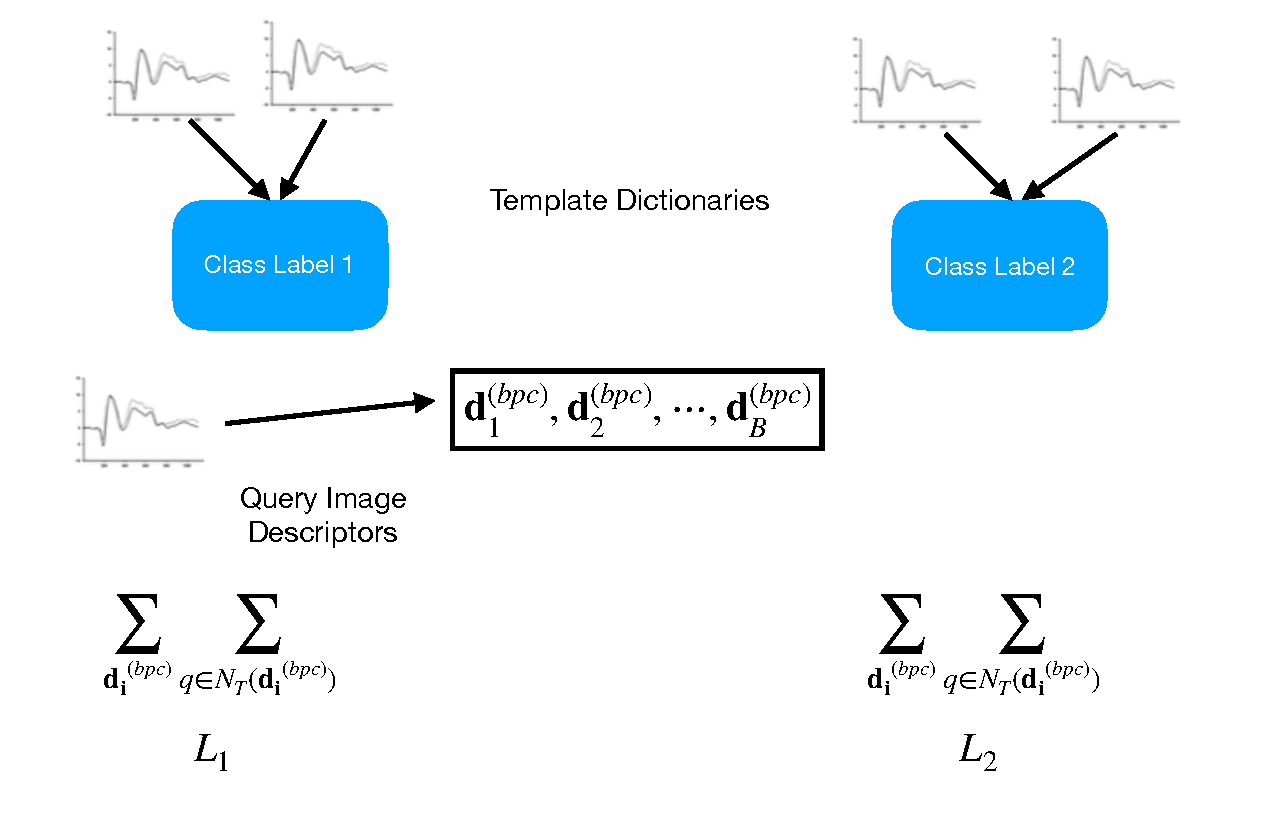
\includegraphics[scale=0.5]{images/Classification1.pdf}
%\caption[Patch Geometry]{(a) Two Dictionaries contain templates descriptors for two different classes. A set of query descriptors are extracted from a new image that needs to be categorized.   }
%\label{fig:nbnnclassification1}
%\end{figure}
%
%
%\begin{figure}[h!]
%\centering
%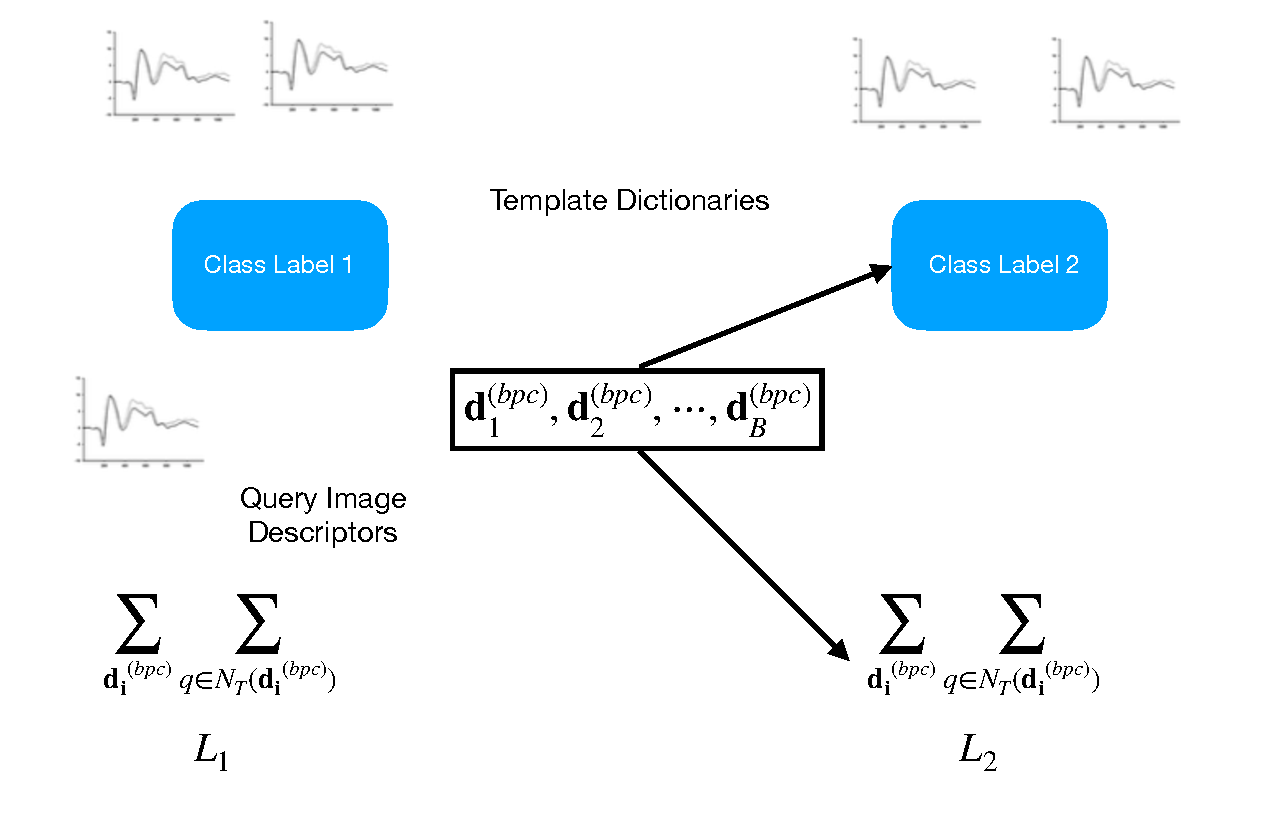
\includegraphics[scale=0.5]{images/Classification2.pdf}
%\caption[Patch Geometry]{(b) Distances from every descriptor $\gls{d}_i$ are calculated against the closest one from the Dictionary of Class 2.  Distances summations are accumulated.  }
%\label{fig:nbnnclassification2}
%\end{figure}
%
%\begin{figure}[h!]
%\centering
%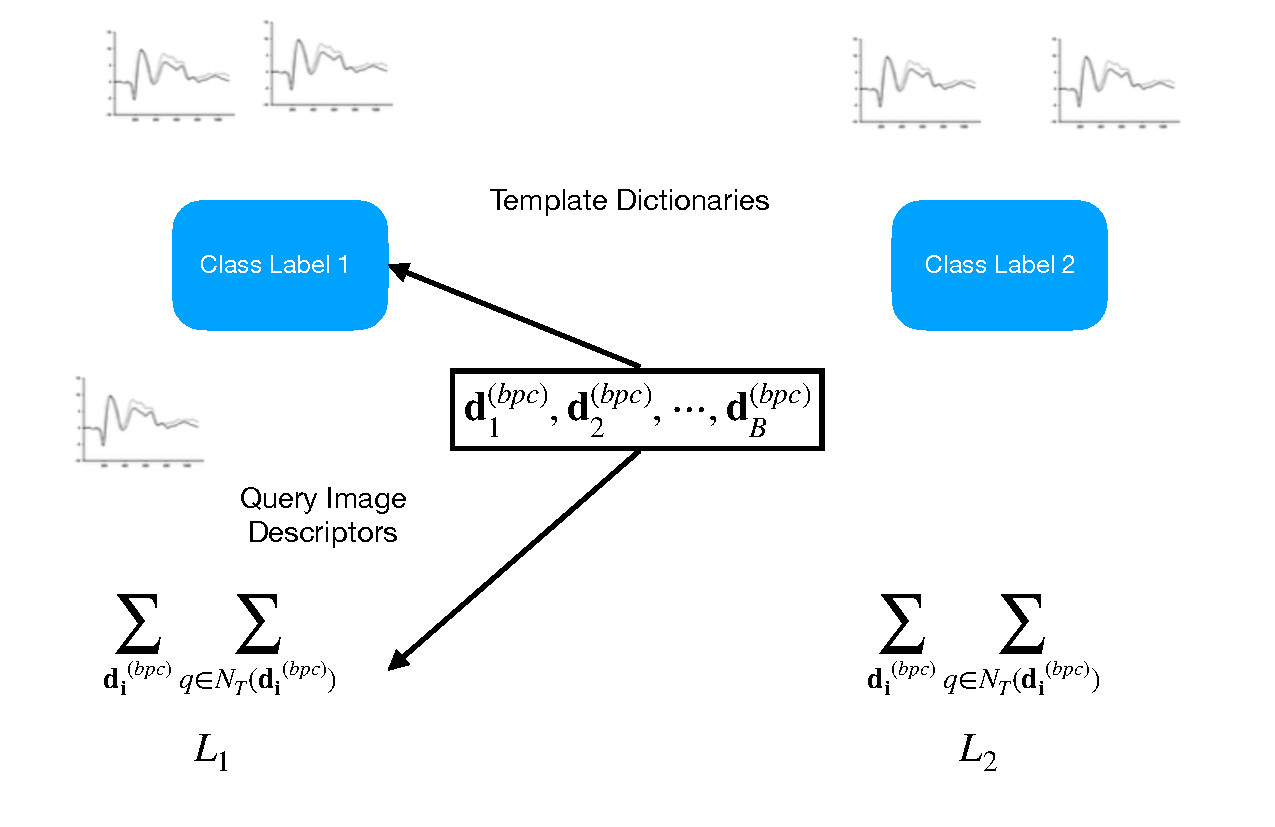
\includegraphics[scale=0.5]{images/Classification3.pdf}
%\caption[Patch Geometry]{(c) Distance values from every descriptor $\gls{d}_i$ are calculated against the closest one from the Dictionary of Class 1.  Distances summations are accumulated.   }
%\label{fig:nbnnclassification3}
%\end{figure}
%
%
%\begin{figure}[h!]
%\centering
%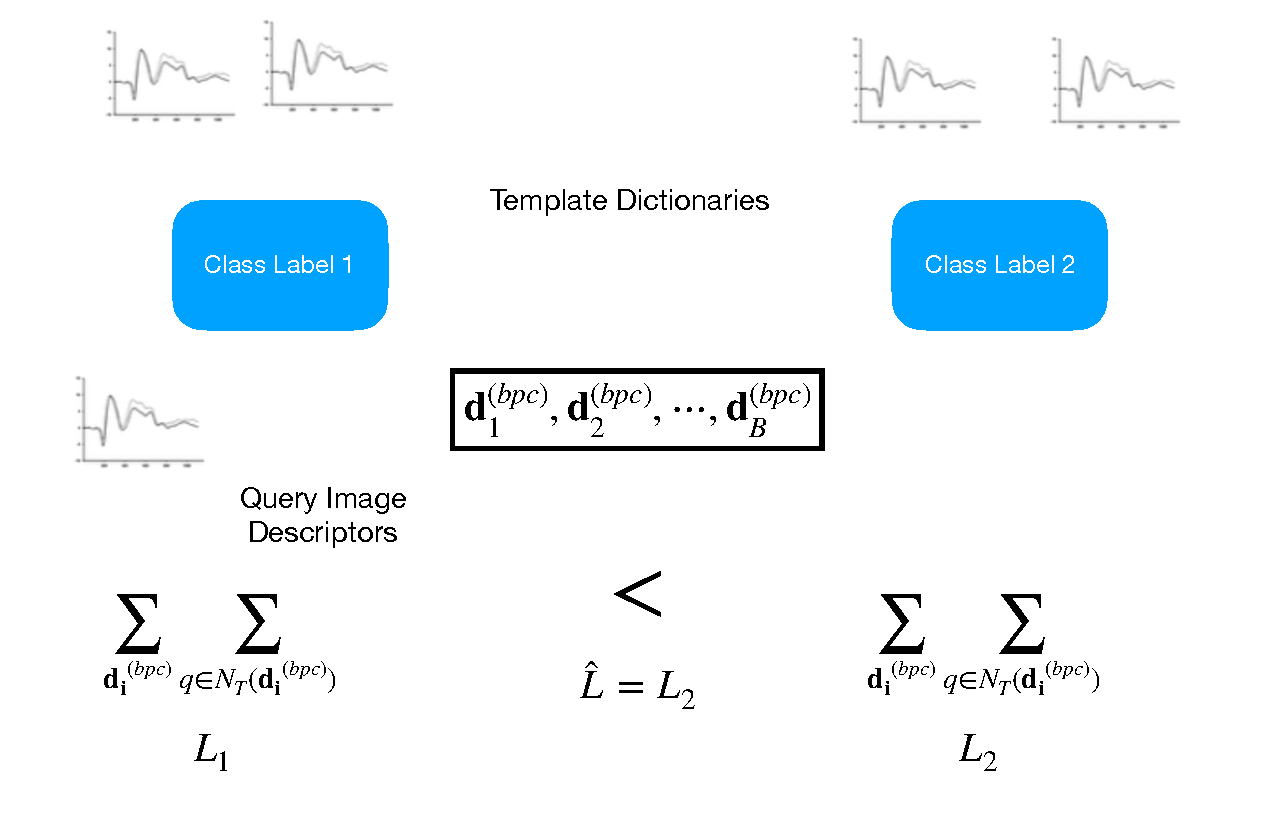
\includegraphics[scale=0.5]{images/Classification4.pdf}
%\caption[Patch Geometry]{(d) The two different summation values are compared against each other. The summation that achieved the lesser value is the one that more closely resembles the set of templates, thus is the one predicted by the classification algorithm.  }
%\label{fig:nbnnclassification4}
%\end{figure}


%TODO Agregar tambien las pruebas sobre rootsift y que la distancia mejor es la coseno demostrar justamente haciendo una prueba sobre EEGWave.
%TODO Agregar que el experimento dio perfecto cuando no se controla la varianza.

\subsection{Algorithm}

In brief, based on segmented signals from at least two labeled classes, a set of images is first generated.  For each image, keypoints are localized and descriptors are extracted during the training or calibration step of a BCI procedure and they are grouped in template dictionaries for each one of the classes.  Additionally, the spatial performance is evaluated and the $\gls{bpc}$ value is computed.

Hence, given a new unlabeled signal segment, an image plot is generated as well, their keypoints localized and their descriptors extracted.  They are fed into Equation~\ref{eq:classification} in order to determine the class which minimizes the summation and thus provide the information bit to the BCI controller.  

\begin{subappendices}

\section{Model Summary}

This section provides a mapping cheat-sheet to convert and obtain the parameters of the algorithm for a given set of signal parameters.

The input signal parameters are $N$,$F_s$, $\lambda$ and the peak-to-peak amplitude $\gls{DeltamuV}$ of the waveform to study. The unit length of the patch is $\Delta_s = \sqrt{2} \; 15$ and as has been earlier mentioned, depends on the particular SIFT implementation.\\


Output parameters are: 
$\gls{gamma}$
$\gls{gammat}$
$\gls{Hy}$
$\gls{Wx}$
$\gls{St}$
$\gls{Sv}$
$\gls{Sy}$
$\gls{Sx}$
$\gls{kp}$\\

Mappings:\\

Time to sample point index conversion

\begin{align*}
n = \left\lfloor F_s \ \Delta_t \right\rfloor \ \gamma_t
\end{align*}

Span of a Patch

\begin{align*}
\Delta_t = \frac{S_t \ \Delta_s}{F_s \ \gamma_t} 
\end{align*}

Amplitude scale factor

\begin{align*}
\gamma = \frac{H_y}{\Delta \mu V}  
\end{align*}

Time scale factor

\begin{align*}
\gamma_t = \frac{W_x}{F_s \; w}  
\end{align*}

Horizontal Patch scale

\begin{align*}
S_t = \frac{ \lambda \;  \  F_s \ \gamma_t }{\Delta_s}
\end{align*}

Vertical Patch scale

\begin{align*}
S_v= \frac{\Delta \mu V \ \gamma}{\Delta_s} 
\end{align*}

Restriction on the horizontal patch scale

\begin{align*}
\frac{W_x-1}{\sqrt{2} \; 15}  \geq S_t 
\end{align*}

Restriction on the vertical patch scale

\begin{align*}
\frac{H_y-1}{\sqrt{2} \; 15}  \geq S_v 
\end{align*}

Horizontal Patch size in pixels

\begin{align*}
\mathbf{S}_x = \lfloor \Delta_s \; S_t \rfloor + 1
\end{align*}

Vertical Patch Size in pixels

\begin{align*}
\mathbf{S}_y = \lfloor \Delta_s \; S_v \rfloor + 1
\end{align*}

Pixel Resolution on the horizontal axis

\begin{align*}
1 P_x \equiv \frac{1}{F_s  \; \gamma_t}  [\si{s}]
\end{align*}

Pixel Resolution on the vertical axis

\begin{align*}
1 P_y \equiv \frac{1}{\gamma}  [\si\mu{V}]
\end{align*}

\end{subappendices}